Even more ubiquitous in astrophysics than accretion onto a single source is accretion between binary systems. This is also where we are able to learn the most about accretion because, by their nature, binary systems reveal more about themselves than individual systems do.
\par
In this section of notes, we'll work through the detailed geometry and dynamics of binary accretion mechanisms, which will lead us toward the theory of disk accretion.

\section{Dynamics of Binary Systems}

Before we dive into the fluid dynamics of binary accretion, we'll first discuss the dynamics of these systems from a gravitational standpoint. There are several important results and will come from this and help along the way later on.

\subsection{The Two-Body Problem}
To understand accretion in binary systems, it’s helpful to briefly recall the dynamics of the classical \textbf{two-body problem}.  We consider two point masses, $M_1$ and $M_2$, interacting only through gravity. Their positions relative to an inertial frame are ${\bf r}_1$ and ${\bf r}_2$, and the vector separating them is  
\[
{\bf r} = {\bf r}_2 - {\bf r}_1.
\]

The equations of motion are
\[
M_1 \ddot{\bf r}_1 = G \frac{M_1 M_2}{r^3} {\bf r}, 
\qquad
M_2 \ddot{\bf r}_2 = -G \frac{M_1 M_2}{r^3} {\bf r}.
\]
Adding these two gives conservation of the \textbf{center of mass (COM)}:
\[
M_1 \ddot{\bf r}_1 + M_2 \ddot{\bf r}_2 = 0 
\quad \Rightarrow \quad 
\ddot{\bf R}_{\rm COM} = 0,
\]
where 
\[
{\bf R}_{\rm COM} = \frac{M_1 {\bf r}_1 + M_2 {\bf r}_2}{M_1 + M_2}.
\]
It is therefore natural to work in the COM frame, where ${\bf R}_{\rm COM} = 0$.  
Defining the \textbf{reduced mass} 
\[
\mu = \frac{M_1 M_2}{M_1 + M_2},
\]
the relative motion reduces to a single particle of mass $\mu$ moving under the potential of the total mass $M = M_1 + M_2$:
\[
\mu \ddot{\bf r} = - \frac{G M_1 M_2}{r^3} {\bf r}
\quad \Rightarrow \quad 
\ddot{\bf r} = - \frac{G M}{r^3} {\bf r}.
\]
Thus, the two-body problem reduces to the motion of a single body in a central potential.  
The orbits are conic sections—elliptical for bound systems—with angular momentum per unit mass
\[
{\bf L} = {\bf r} \times \dot{\bf r},
\]
and total specific energy
\[
E = \frac{1}{2}\dot{r}^2 - \frac{GM}{r}.
\]
While this is a fairly elementary problem to solve and is well known to most astronomy students, it is worth noting that our standard intuition for orbits must be stretched somewhat in this case. We now recognize that it is the \textbf{separation} between the two bodies which follows a standard elliptical orbit and that we must be careful not to mistake our intuition for planetary orbits with those here.
\par
Now, the \textbf{main observable of a binary is the period}, therefore, we will use that to determine other properties. Using \textbf{Kepler's Law},
\[
a^3 = \frac{GM_{\rm tot}}{4\pi^2} P^2.
\]
\rmk{It's worth remembering here that this is the \textit{relative orbit} in the equivalent 1-body problem. Thus, its the proper distance \textit{between the companions}, but it is NOT the orbital radius.}
We will also find it convenient to introduce the \textbf{mass ratio} $q = M_2/M_1$. We may write $a$ in terms of the mass ratio and the period as
\begin{equation}
\label{eq:binary_orbit_semi_major_axis}
\boxed{
    a = \left(\frac{G}{4\pi^2}\right)^{1/3} M_1^{1/3}(1+q)^{1/3} P^{2/3}.
}
\end{equation}
In units of solar masses, this reduces to
\begin{equation}
    \label{eq:binary_orbit_semi_major_axis_united}
    \boxed{
    a = \begin{cases}
        1.5\times 10^{13} \left(\frac{M_1}{M_\odot}\right)^{1/3} (1+q)^{1/3} P_{\rm years}^{2/3}\; {\rm cm},&\\
                2.9\times 10^{11} \left(\frac{M_1}{M_\odot}\right)^{1/3} (1+q)^{1/3} P_{\rm days}^{2/3}\; {\rm cm},&\\
                        3.5\times10^{10} \left(\frac{M_1}{M_\odot}\right)^{1/3} (1+q)^{1/3} P_{\rm hrs}^{2/3}\; {\rm cm},&\\
    \end{cases}
    }
\end{equation}
\begin{remark}
    Notice that $q > 0$ no matter what, so we always know that leaving out the $1+q$ term provides a \textbf{lower bound} on $a$. In principle, $q \to \infty$ can occur, in which case $a \to \infty$; however, this isn't really relevant in practice.
\end{remark}

In the COM frame, the distance to each of the companions is determined by the fact that ${\bf r} = {\bf r}_1 - {\bf r}_2 = a$, which means that (\rmk{easy enough to work this out from the definition of the COM}),
\[
{\bf r}_1 = \frac{M_2}{M_1+M_2} {\bf r},\; {\bf r}_2 = - \frac{M_1}{M_1+M_2} {\bf r}.
\]
In terms of $q$, 
\[
{\bf r}_1 = \frac{1}{1+q} {\bf r},\; {\bf r}_2 = - \frac{q}{1+q} {\bf r}.
\]


\subsection{Tidal Forces in Binary Systems}

One important feature of accreting binaries is that they are \textbf{close binaries}: therefore, we cannot ignore the role that tidal forces play in the dynamics. This serves two really important purposes which we will exploit in developing the theory:

\begin{enumerate}
    \item Tidal forces \textbf{circularize binary orbits}, and
    \item tidal forces \textbf{synchronize axial rotations}.
\end{enumerate}

To understand these phenomena, we consider a qualitative picture: Let $M_1$ and $M_2$ be the masses of two stars in binary orbit. If $M_1$ experiences tidal distortion, it will bulge along the \textit{line of centers}. Now, the star is also rotating, which means that the bulge will need to shift backward to align with the line of centers. In a perfectly elastic star, this shift could happen rapidly, but that is not generally the case. 
\par
As a result, the tidal bulge tends to either lead or follow the \textit{line of centers}, which means that the COM of the star is shifted either forward or backward in the orbit. If it is shifted backward, then the companion will pull it forward, slowing the rotation and increasing the angular momentum in the orbit to match. Likewise, if it is shifted forward, it will be pulled backward and the rotation will increase and angular momentum will be pulled out of the orbit. Internally, this rearranging of material will lead to dissipative processes which serve to reduce the overall energy of the orbit to the minimum possible for a given fixed angular momentum. This will correspond to synchronous rotation of the binaries and circular orbits.
\par
In general, this process is quite efficient:
\[
t_{\rm tide} \sim \left(\frac{a}{R}\right)^5\;\text{or faster},
\]
where $a$ is the semi-major axis of the orbit and $R$ is the radius of the tidally effected star. It is therefore \textit{generally} the case that these evolutions occur on time scales short relative to the timescale of accretion.
\rmk{(This is not \textit{always} the case: there are exceptions!)}
\paragraph{Implications}
The result of this is that, for most relevant systems, we can treat the problem of accretion in a somewhat simpler scenario: we have circular, Keplerian orbits and the systems are tidally locked. This means that in a frame centered on the COM and co-rotating with the orbit, the bodies appear to be \textbf{stationary}.

\subsection{The Restricted 3-Body Problem}

Having established the dynamics of the two companion stars, we now ask a natural question:
\vspace{0.25cm}
\begin{center}
    \textit{What is the motion of a test particle released in the combined gravitational field of the two companions?}
\end{center}
\vspace{0.25cm}

To study this problem, we work in the \textbf{co-rotating center-of-mass frame}. In this frame, the two companions remain \textbf{fixed} at their orbital radii and appear \textbf{non-rotating}. The tradeoff is that we must introduce the \textbf{fictitious forces} associated with the non-inertial frame. Defining the rotational velocity vector
\[
\boldsymbol{\Omega} = \Omega \hat{\bf z} 
= \left(\frac{GM}{a^3}\right)^{1/2}\hat{\bf z},
\]
the fictitious accelerations are:
\vspace{0.5cm}
\begin{enumerate}
    \item \textbf{Coriolis Force}: ${\bf F}_{\rm cor} = -2m\, \boldsymbol{\Omega} \times \dot{\bf r}$,
    \item \textbf{Centrifugal Force}: ${\bf F}_{\rm cent} = -m\, \boldsymbol{\Omega} \times (\boldsymbol{\Omega} \times {\bf r})$,
    \item \textbf{Euler Force}: ${\bf F}_{\rm Euler} = -m\, \dot{\boldsymbol{\Omega}} \times {\bf r}$.
\end{enumerate}
\vspace{0.5cm}

For binaries of constant orbital period, $\dot{\boldsymbol{\Omega}}=0$, so the Euler force can be neglected. The Euler equation in the rotating frame becomes
\[
\frac{D{\bf u}}{Dt} = - \frac{\nabla P}{\rho} - \nabla \Phi_{\rm Roche} - \underbrace{2 \boldsymbol{\Omega} \times \dot{\bf r}}_{\text{Coriolis Force}},
\]
where $\Phi_{\rm Roche}$ is the combined gravitational and centrifugal potential, called the \textbf{Roche Potential}:
\begin{equation}
    \label{eq:roche_potential}
    \boxed{
    \Phi_{\rm Roche} =
    - GM_2 \left[\frac{1}{q|{\bf r} - {\bf r}_1|} + \frac{1}{\,|{\bf r}-{\bf r}_2|}\right]
    - \tfrac{1}{2}\left|\boldsymbol{\Omega}\times{\bf r}\right|^2
    }.
\end{equation}

\begin{figure}
    \centering
    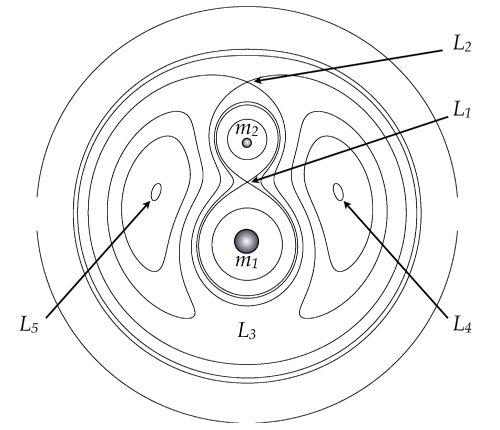
\includegraphics[width=0.75\linewidth]{Pictures/figures/roche_potential.png}
    \caption{The Roche potential in the orbital plane for a representative mass ratio. Equipotential contours illustrate the balance between gravitational and centrifugal forces in the co-rotating frame.}
    \label{fig:roche_potential}
\end{figure}

\subsubsection{Lagrange Points}

Inspection of the Roche potential (Figure~\ref{fig:roche_potential}) reveals the existence of \textbf{five equilibrium points}, known as the \textbf{Lagrange points}. At these locations, the effective force vanishes in the co-rotating frame. Of these, the most important for mass transfer is the inner point, $L_1$, located between the two stars. This is a \textbf{saddle point} of the potential and defines the boundary between the two \textbf{Roche lobes}. Material within a lobe is gravitationally bound to its host star, while material near $L_1$ can pass through to the companion. 

In two dimensions, the Roche lobes take the form of a figure-eight, while in three dimensions they resemble a dumbbell (Figure~\ref{fig:roche_lobes}). The geometry of these lobes determines when a star will begin to lose mass through Roche lobe overflow.

\begin{figure}
    \centering
    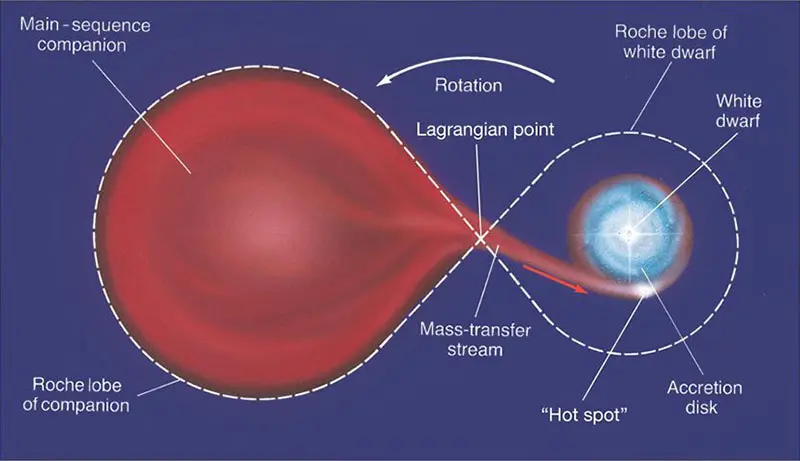
\includegraphics[width=0.75\linewidth]{Pictures/figures/roche_lobes.png}
    \caption{The Roche lobes of two stars in a binary, shown as equipotential surfaces of the Roche potential. The $L_1$ point at the intersection of the lobes sets the critical condition for Roche lobe overflow.}
    \label{fig:roche_lobes}
\end{figure}

\section{Roche Lobe Overflow}

We now discuss the nature of material accreted onto a companion from a progenitor star. Consider the scenario given above when the radii of the individual companions ($R_1$ and $R_2$) are each much, much smaller that their respective Roche Lobes. From the Euler Equation,
\[
\frac{D{\bf u}}{Dt} = - \frac{\nabla P}{\rho} - \nabla \Phi_{\rm Roche} - 2 \boldsymbol{\Omega} \times {\bf u},
\]
we see that in steady state,
\[
0 = - \frac{\nabla P}{\rho} - \nabla \Phi_{\rm Roche},
\]
which implies that the surface (defined by $\nabla P = 0$) will coincide with one of the inner most equipotentials deep within the respective Roche lobe. What do we learn from this? \textbf{For binaries which are each deep within their own Roche Lobes, there is no impetus for mass transfer.} Such binaries are called \textbf{detached binaries}.
\par
Now we might consider another scenario where one companion (the so-called \textbf{secondary} or \textbf{non-accretor}) expands (due to any number of relevant processes) such that it begins to fill its Roche Lobe. Here's the critical idea:
\vspace{0.25cm}
\begin{center}
    When material on the surface (which is on equipotentials of $\Phi_{\rm Roche}$) begins to fill the Roche-Lobe, that material will lie close to the $L_1$ point. In turn, perturbations can \textbf{displace material across $L_1$ into the corresponding Roche Lobe of the primary WITHOUT needing additional energy input.} 
\end{center}
\vspace{0.25cm}
Such binaries are called \textbf{semi-detached binaries} and are able to efficiently transfer mass across the $L_1$ point. Another interesting scenario occurs when both objects fill their Roche-Lobes, creating a so-called \textbf{contact binary}.
\begin{remark}
    It will be seen that the rate of material flow is quite fast. As such, we rarely get a companion which is much larger than its own Roche Lobe.
\end{remark}

\subsection{Geometry of Binary Accretion}

Before we can work out the details of binary accretion, we'll need to do a bit of geometry. Our goal here is to answer the following general questions:
\vspace{10pt}
\begin{enumerate}
    \item \textbf{Where} is the L1 point relative to the primary in a binary system?
    \item \textbf{How big} is the Roche Lobe for a given mass?
    \item \textbf{What} determines the size and shape of the Roche Lobe?
\end{enumerate}
\vspace{10pt}
\medskip
\par
Looking again at the equation for the Roche Potential, we have \eqref{eq:roche_potential}
\[
    \Phi_{\rm Roche} =
    - GM_2 \left[\frac{1}{q|{\bf r} - {\bf r}_1|} + \frac{1}{\,|{\bf r}-{\bf r}_2|}\right]
    - \tfrac{1}{2}\left|\boldsymbol{\Omega}\times{\bf r}\right|^2.
\]
If we imagine that the binary orbit is circular, then their distance is determined unambiguously from their period (or, conversely, their period is determined from their distance). As such, we see that there are only really two major ingredients in determining the scale and shape of the Roche Lobes:
\vspace{10pt}
\begin{enumerate}
    \item The \textbf{separation} determines a scale for the Roche Geometry,
    \item The \textbf{mass ratio} determines the shape of the geometry.
\end{enumerate}
\vspace{10pt}
The implication here is quite clear: we \textbf{should} be able to say a great deal about the geometry of the Roche System without a direct reference to anything other than $q$. Unfortunately, it is generally a task requiring numerical solution, but there are some quasi-analytic formulae which will be relevant to our discussion of these phenomena.

\subsubsection{The Roche Lobe Radius}

One such option is the \textbf{Eggleton Formula}, which dictates the \textbf{shape of the Roche Lobe} as a function of the mass ratio $q$. It is a numerical fit to computation data taking the form:
\begin{equation}
\label{eq:eggleton_formula}
\boxed{
    \frac{R_2}{a} = \frac{\alpha q^{2/3}}{\beta q^{2/3} + \log(1+q^{1/3})}
    }
\end{equation}
where $\alpha = 0.49$, and $\beta = 0.6$. \rmk{We can get at $R_1$ from replacing $q$ with $q^{-1}$.} Here, $R_2$ is the \textit{effective radius} of the lobe defined as the radius of a sphere with the \textit{same volume as the lobe.} There are also two other approximations worthy of mention:

\begin{enumerate}
    \item $(0.1 \le q \le 0.8)$: We can use a simplified version from \citet{1971ARA&A...9..183P}:
    \begin{equation}
        \label{eq:paczynski_lobe_radius}
        \boxed{
        \frac{R_2}{a} = \frac{2}{3^{4/3}}\left(\frac{q}{1+q}\right)^{1/3} = 0.462\left(\frac{M_2}{M_1+M_2}\right)^{1/3}.}
    \end{equation}
This proves to be a \textbf{massively important} equation because it permits us to discuss many different scaling relationships for different types of primaries and secondaries.
    \item $(0.03 < q < 1)$ also allows
\[
\frac{R_1}{R_2} = \left(\frac{M_1}{M_2}\right)^{0.45}.
\]

\end{enumerate}

\subsubsection{The Location of the Lagrange Point}

We are also interested in the distance between the \textit{primary} (the accretor) and the Roche-Lobe critical point. To good accuracy, a fitted formula suffices \citep{1964BAICz..15..165P}:
\begin{equation}
    \label{eq:roche_overflow_distance}
    \frac{b_1}{a} = 0.5 - 0.227 \log q,
\end{equation}
where $a$ is the semi-major axis (the distance between the primary and the secondary due to circularization) and $b_1$ is the distance between the primary and the Roche point. Clearly, for $q = 1$, the Roche point is right between the primary and the secondary. For $q \gg 1$ (corresponding to a low mass accretor and high mass donor), the overflow point get \textbf{closer to the primary} since the secondary can bind material more effectively. In the opposite scenario, $q \ll 1$, the overflow point gets closer to the secondary. To \textbf{first order} in $q$, this is
\[
\frac{b_1}{a} \approx 0.5 - 0.227(q-1).
\]
\subsection{Scaling Relations for Roche Lobe Overflow}

One of the most useful aspects of equation~\eqref{eq:paczynski_lobe_radius} is that it expresses the Roche–lobe radius $R_2$ entirely in terms of the binary separation $a$ and the mass ratio $q = M_2 / M_1$.  
Using Kepler’s Third Law, we can replace the separation by the observable orbital period $P$:
\begin{equation}
a = \left[\frac{G (M_1 + M_2)}{4\pi^2}\right]^{1/3} P^{2/3}.
\end{equation}
Substituting into the Roche–lobe relation gives
\begin{align}
R_2 &\approx a\,\frac{2}{3^{4/3}} \left(\frac{q}{1+q}\right)^{1/3} \\[4pt]
&= \frac{2}{3^{4/3}}\!\left(\frac{G}{4\pi^2}\right)^{1/3}
   P^{2/3} (M_1 + M_2)^{1/3}
   \left(\frac{M_2}{M_1 + M_2}\right)^{1/3} \\[4pt]
&= \frac{2}{3^{4/3}}\!\left(\frac{G}{4\pi^2}\right)^{1/3}
   P^{2/3} M_2^{1/3}.
\end{align}
Thus, to good approximation, the Roche–lobe radius of the donor depends only on its own mass and the binary period.  
Evaluating the constants yields the very useful scaling:
\[
\boxed{
R_2 \simeq 6.2 \times 10^{11}
\left(\frac{P}{{\rm 1\,day}}\right)^{2/3}
\left(\frac{M_2}{M_\odot}\right)^{1/3}
{\rm cm}.
}
\]

\subsubsection{The Period–Density Relation}

Since a Roche–lobe filling star must satisfy this radius–period relation, its mean density follows immediately:
\begin{equation}
\bar{\rho} = \frac{3M_2}{4\pi R_2^3}.
\end{equation}
Substituting for $R_2$, we find
\begin{align}
\bar{\rho} 
   &\sim \frac{3M_2}{4\pi}
      \left[\frac{3^{4/3}}{2}
      \left(\frac{4\pi^2}{G}\right)^{1/3}
      P^{-2/3} M_2^{-1/3}\right]^3 \\[4pt]
   &= \frac{3^5 \pi}{8 G P^2}.
\end{align}
Hence the donor’s mean density depends \emph{only on the orbital period}, not on the stellar mass or composition:
\[
\boxed{
\bar{\rho} \;\approx\; 110\,P_{\rm hr}^{-2}\;{\rm g\,cm^{-3}},
}
\]
where $P_{\rm hr}$ is the orbital period in hours.

\medskip
\noindent
\textbf{Physical meaning:} systems with shorter periods must contain denser donors.  
This simple $P^{-2}$ scaling makes the orbital period a direct diagnostic of the donor’s mean density—and thus its evolutionary state.

\subsubsection{The Mass–Period Relation for Polytropic Donors}

If the donor follows a polytropic structure with index $n$, then
\begin{equation}
R \propto M^{\frac{1-n}{3-n}},
\end{equation}
and the corresponding mean density is
\begin{equation}
\bar{\rho} \propto M^{\tfrac{3n}{3-n}}.
\end{equation}
Since Roche–lobe filling enforces $\bar{\rho} \propto P^{-2}$, we obtain the general
\textbf{mass–period relation}:
\[
\boxed{
P \propto M^{-\tfrac{3n}{2(3-n)}}.
}
\]

\paragraph{Main Sequence Donors}
For main sequence stars, an empirical relation $R \propto M^{3/4}$ is a good approximation.  
Then
\begin{align}
\bar{\rho}
   &= \frac{3M}{4\pi R^3}
   \approx 1.4
   \left(\frac{M}{M_\odot}\right)^{-5/4}
   {\rm g\,cm^{-3}},
\end{align}
and equating with $\bar{\rho} \approx 110\,P_{\rm hr}^{-2}$ gives
\[
P_{\rm hr} \approx 8.8
\left(\frac{M}{M_\odot}\right)^{5/8},
\qquad
\boxed{
\frac{M}{M_\odot} \approx 0.03\,P_{\rm hr}^{8/5}.
}
\]
Because main sequence stars cannot exist below about $0.1\,M_\odot$, this relation implies a lower limit near 
$P_{\rm min} \sim 2\,{\rm hr}$—shorter-period systems must therefore contain evolved or degenerate donors.

\paragraph{Degenerate Donors}
For fully degenerate (non-relativistic) donors, $R \propto M^{-1/3}$, so that
\[
\bar{\rho} \propto M^{2},
\qquad
P \propto M^{-1}.
\]
Hence more massive degenerate donors correspond to shorter orbital periods.  
A typical scaling is
\[
\boxed{
P_{\rm sec} \approx 150
\left(\frac{M}{M_\odot}\right)^{-1},
}
\]
appropriate for low-mass white dwarf donors.

\subsubsection{The Minimum Period in Compact Binaries}

These two contrasting mass–period scalings explain the observed \textbf{period bounce} in compact binaries:
\begin{itemize}
    \item For \textbf{main sequence donors} ($R \propto M^{3/4}$):  
    $P \propto M^{8/5}$, so as mass is lost, the orbital period \emph{decreases}.
    \item For \textbf{degenerate donors} ($R \propto M^{-1/3}$):  
    $P \propto M^{-1}$, so further mass loss causes the period to \emph{increase}.
\end{itemize}
The system therefore evolves toward shorter periods until the donor becomes degenerate, reaches a minimum period, and then expands again.  
This transition defines the \textbf{minimum orbital period}:
\[
P_{\rm min} \sim 1\,{\rm hr}, 
\qquad
M_2 \sim 0.03\text{--}0.04\,M_\odot.
\]

\begin{bigidea}
\textbf{Key Concepts}
\begin{itemize}
    \item The Roche–lobe size depends only on the mass ratio $q$ and separation $a$.
    \item For a Roche–lobe filling star, the \textbf{mean density depends solely on the orbital period}:
    \[
    \bar{\rho} \approx 110\,P_{\rm hr}^{-2}\;{\rm g\,cm^{-3}}.
    \]
    \item Combining this with stellar structure relations $R(M)$ gives characteristic \textbf{mass–period laws}:
    \begin{itemize}
        \item \textbf{Main sequence donors:} $P_{\rm hr} \approx 8.8(M/M_\odot)^{5/8}$.
        \item \textbf{Degenerate donors:} $P_{\rm sec} \approx 150(M/M_\odot)^{-1}$.
    \end{itemize}
    \item The \textbf{period bounce} arises where these two regimes meet, marking the transition from main sequence to degenerate donors.
\end{itemize}
\end{bigidea}

\subsection{The Evolution of Binary Systems}

The evolution of a binary system is governed by the exchange of two fundamental quantities:
\textbf{mass} and \textbf{angular momentum}.  
Any process that redistributes or removes either quantity inevitably alters the orbital configuration of the system—often in a way that feeds back on the rate and stability of mass transfer itself.

\par
In most cases, we begin by assuming \textbf{conservative mass transfer}, in which the mass lost by the donor (secondary) is entirely accreted by the companion (primary). However, it is not always valid to assume that the system’s \textbf{angular momentum} is likewise conserved. Angular momentum losses can profoundly affect the orbital evolution and often determine whether mass transfer proceeds stably or becomes dynamically unstable.

\begin{definition}[Fully Conservative Mass Transfer]
\textbf{Fully conservative mass transfer} refers to the idealized case in which both the total mass and the total angular momentum of the binary are conserved:
\[
\dot{M}_1 + \dot{M}_2 = 0, \qquad \dot{J} = 0.
\]
In this limit, all material lost by the donor is accreted by the companion, and no angular momentum escapes the system.
\end{definition}

\par
In reality, few binaries are perfectly conservative.  Mass and angular momentum can be lost through several mechanisms—most notably through \textbf{gravitational wave radiation}, \textbf{stellar winds}, or \textbf{magnetically driven outflows}.  These processes remove energy and angular momentum from the orbit, driving secular changes in the separation and period that ultimately shape the system’s long-term evolution.
\medskip
\noindent
As we will see in the sections that follow, the coupled transfer of mass and angular momentum governs the fate of a binary system—determining whether it expands or contracts, remains stable, or undergoes runaway mass transfer leading to a common-envelope phase.

\subsubsection{The Role of Angular Momentum}

Given an orbital period $P$ and angular velocity $\omega = 2\pi / P$, the total orbital angular momentum is
\[
J = (M_1 a_1^2 + M_2 a_2^2)\,\omega,
\]
where $a_1$ and $a_2$ are the distances of each component from the center of mass:
\[
a_1 = \frac{M_2}{M_1 + M_2}a,
\qquad
a_2 = \frac{M_1}{M_1 + M_2}a.
\]
Substituting these expressions and invoking Kepler’s third law,
\[
\omega^2 a^3 = G(M_1 + M_2),
\]
we obtain the compact and widely used form:
\[
\boxed{
J = M_1 M_2 \left(\frac{G a}{M_1 + M_2}\right)^{1/2}.
}
\]
If we now take the \textbf{logarithmic derivative} of the above equation, we find after requiring \textbf{conservative mass transfer} that
\begin{equation}
    \label{eq:ang_mom_binary_ev}
\frac{\dot{a}}{a} = \frac{2\dot{J}}{J}
    + 2\frac{(-\dot{M}_2)}{M_2}\left(1 - \frac{M_2}{M_1}\right),
\end{equation}
which leads us immediately to a big idea:
\begin{bigidea}

Equation~\eqref{eq:ang_mom_binary_ev} shows how the \textbf{orbital separation $a$} responds to changes in angular momentum and mass transfer! From this expression, we can immediately draw several key conclusions:
\begin{itemize}
    \item If \textbf{angular momentum is conserved} ($\dot{J}=0$):
    \begin{itemize}
        \item When $M_2 < M_1$, the factor $(1 - M_2/M_1)$ is positive, so $\dot{a} > 0$.  
        The orbit \textbf{expands} as the lighter donor transfers mass to the heavier accretor.
        \item When $M_2 > M_1$, the factor $(1 - M_2/M_1)$ is negative, so $\dot{a} < 0$.  
        The orbit \textbf{shrinks} as the more massive star loses mass to its lighter companion.
    \end{itemize}
    \item If \textbf{angular momentum is lost} ($\dot{J}<0$), this term always contributes to orbital contraction, regardless of the mass ratio.  
\end{itemize}
An intuitive way to think about this is in the limit $q \gg 1$, in which case we are just adding mass or removing mass from a mass on a string. If we add mass, we would need to swing harder
to keep it at the same distance, or we would shorten the string. Likewise, if we remove mass, it will want to drift outward.
\end{bigidea}

\medskip
\paragraph{Angular Momentum Loss Channels.}
In the idealized \emph{fully conservative} case, the total angular momentum of the system is conserved ($\dot{J}=0$).  
However, in realistic binaries, a variety of processes can remove angular momentum from the orbit.  
These losses drive secular changes in the orbital separation and can dramatically influence the stability of mass transfer.  
The most important loss mechanisms are summarized below.

\begin{itemize}
    \item \textbf{Gravitational Radiation.}  
    Compact binaries (white dwarfs, neutron stars, black holes) emit gravitational waves as they orbit, carrying away angular momentum at a rate
    \[
    \dot{J}_{\rm GW} = -\frac{32}{5}\frac{G^{7/2}}{c^5}
        \frac{M_1^2 M_2^2 (M_1 + M_2)^{1/2}}{a^{7/2}}.
    \]
    This loss steeply depends on $a^{-7/2}$, making gravitational radiation dominant only in very tight systems.  
    The resulting orbital decay leads to a gradual inspiral, eventually producing a merger or the onset of Roche–lobe overflow.

    \item \textbf{Magnetic Braking.}  
    In systems containing late-type (cool, convective) stars, magnetic fields can couple the stellar wind to the star’s rotation.  
    The wind carries away angular momentum from the spin of the donor, which is tidally locked to the orbit.  
    As a result, the \emph{orbital} angular momentum also decreases.  
    The torque can be approximated by empirical laws such as
    \[
    \dot{J}_{\rm MB} \propto - M_2 R_2^{4} \omega^{3},
    \]
    though the efficiency depends strongly on the magnetic field geometry and wind strength.  
    Magnetic braking is a key driver of orbital evolution in cataclysmic variables and low-mass X-ray binaries.

    \item \textbf{Stellar Winds and Outflows.}  
    When one or both stars lose mass in a stellar wind, the escaping gas carries with it specific angular momentum.  
    The total angular momentum loss depends on where the mass leaves:
    \[
    \dot{J}_{\rm wind} \sim \dot{M}_{\rm loss}\, a^2 \omega.
    \]
    If the lost material escapes isotropically from the system, the orbit typically \emph{expands}; if it leaves preferentially through $L_2$ or in a focused jet, it can instead lead to orbital contraction.

    \item \textbf{Mass Loss through $L_2$ or a Circumbinary Disk.}  
    When transfer through $L_1$ becomes excessive, material may flow out through the outer Lagrange point $L_2$, forming a circumbinary ring or disk.  
    Because this ejected matter orbits at larger radii, it extracts \emph{more} specific angular momentum per unit mass than the binary average, leading to rapid orbital decay and possibly a common-envelope phase.

    \item \textbf{Tidal Torques and Spin–Orbit Coupling.}  
    In close systems, tidal interactions exchange angular momentum between the stellar spins and the orbit.  
    Tidal friction tends to synchronize rotation and circularize the orbit.  
    If either star contracts or expands (changing its moment of inertia), this coupling can further exchange angular momentum with the orbit.
\end{itemize}

\paragraph{Consequences of Angular Momentum Loss.}
All of these processes modify the orbital separation through the relation
\[
\frac{\dot{a}}{a} = \frac{2\dot{J}}{J}
    - 2\frac{\dot{M}_2}{M_2}\left(1 - \frac{M_2}{M_1}\right),
\]
which shows that $\dot{J}<0$ always drives orbital contraction.  
In compact systems, this can bring the stars into contact and trigger Roche–lobe overflow, while in wider systems it may gradually shrink the orbit over gigayear timescales.

\begin{bigidea}
\textbf{Angular Momentum Loss Summary}
\begin{itemize}
    \item \textbf{Gravitational waves} dominate at small separations ($a \lesssim R_\odot$).
    \item \textbf{Magnetic braking} dominates for cool, magnetized donors in wider binaries.
    \item \textbf{Winds and circumbinary mass loss} remove angular momentum at intermediate scales and often govern long-term orbital evolution.
    \item \textbf{Tidal coupling} redistributes angular momentum between spin and orbit, enforcing synchronization and circularization.
\end{itemize}
Together, these mechanisms determine whether a binary will widen, shrink, or merge—and hence whether it becomes a stable accretor, a contact binary, or a gravitational wave source.
\end{bigidea}

\subsection{Mass Transfer Stability}
\begin{figure}[ht!]
    \centering
    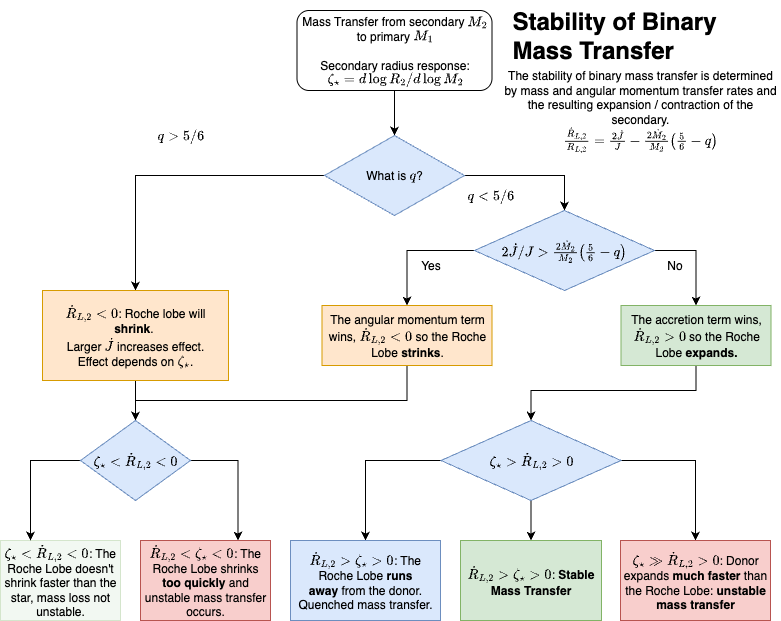
\includegraphics[width=1\linewidth]{Pictures/figures/binary_mass_accretion.png}
    \caption{The various modes of binary mass transfer and the resulting stability as dictated by the stellar contraction response, $\zeta_\star$ and the contraction of the donor Roche Lobe. This is characterized by equation~\eqref{eq:roche_lobe_stability}.}
    \label{fig:roche_transfer_stability}
\end{figure}

Let's now ask the following question: \textbf{what happens to the Roche Lobe when mass is transferred?} 
From equation~\eqref{eq:paczynski_lobe_radius}, we can logarithmically differentiate to find
\[
\boxed{
\frac{\dot{R}_2}{R_2} = \frac{\dot{a}}{a} + \frac{\dot{M}_2}{3M_2},
}
\]
which can then be substituted into \eqref{eq:ang_mom_binary_ev} to obtain
\begin{equation}
\label{eq:roche_lobe_stability}
\boxed{
    \frac{\dot{R}_2}{R_2} = \frac{2\dot{J}}{J} - \frac{2\dot{M}_2}{M_2}\left(\frac{5}{6}-\frac{M_2}{M_1}\right).
}
\end{equation}
\par
We can now interpret equation~\eqref{eq:ang_mom_binary_ev}
together with the Roche lobe response.  The key diagnostic is
\[
\frac{\dot{R}_2}{R_2} = \frac{2\dot{J}}{J}
   + \frac{2(-\dot{M}_2)}{M_2}\!\left(\frac{5}{6} - \frac{M_2}{M_1}\right),
\]
which measures how the Roche lobe of the donor responds as mass is lost.

\begin{enumerate}
    \item \textbf{Unstable (Cataclysmic) Mass Transfer, $q > 5/6$:}  
    In this regime the second term on the right--hand side is negative.  
    If there is any angular momentum loss ($\dot{J}<0$), the Roche lobe shrinks as material is lost.  
    The donor thus overfills its Roche lobe more and more, leading to a runaway process.  
    This behavior underlies cataclysmic variables and other explosive transfer scenarios.

    \item \textbf{Stable Mass Transfer, $q < 5/6$:}  
    Here the second term tends to be positive, so the Roche lobe expands as mass is removed.  
    Provided angular momentum loss is not too strong, the Roche lobe expansion can keep pace with 
    the donor’s radius, allowing for long--lived, secular mass exchange on nuclear or thermal timescales.  

    \item \textbf{Role of Angular Momentum Loss:}  
    Even for $q > 5/6$, strong angular momentum loss (e.g.\ by gravitational radiation or magnetic braking) 
    can still cause the Roche lobe to contract, destabilizing the system.  
    Conversely, with $\dot{J}=0$ and $q > 5/6$, mass transfer remains stable.
\end{enumerate}

\noindent
Thus the fate of the binary depends jointly on the \emph{mass ratio} and the \emph{angular momentum loss channels}:  
low-$q$ systems tend toward runaway transfer, while high-$q$ systems may support stable, long-lived exchange.

\begin{bigidea}
    From the discussion above, we have two very useful criteria which tell us \textbf{a lot} about the nature of our accretion.
    \begin{enumerate}
        \item The equation
            \[ 
            \frac{\dot{a}}{a} = \frac{2\dot{J}}{J} - \frac{2 \dot{M}_2}{M_2} \left(1-\frac{M_2}{M_1}\right)
            \]
            derived above gives us a clear threshold for the \textbf{expansion / contraction} of the orbits:
            \begin{itemize}
                \item If $M_2>M_1$, then the orbit will \textbf{shrink}.
                \item If $M_1 > M_2$, then the orbit will \textbf{expand}.
            \end{itemize}
            Thus, the stability of the binary depends crucially on the initial mass ratio.
        \item Using the Paczyński approximation, we also know that 
        \[
        \frac{\dot{R}_2}{R_2} = \frac{2\dot{J}}{J} - \frac{2\dot{M}_2}{M_2}\left(\frac{5}{6}-\frac{M_2}{M_1}\right),
        \]
        which tells us how the Roche lobe radius evolves relative to the donor mass. 
        \begin{itemize}
            \item If $\frac{M_2}{M_1} < \tfrac{5}{6}$, then (because $\dot{M}_2 < 0$), the second term on the RHS provides a \textbf{positive contribution} and therefore generally leads to Roche Lobe \textbf{expansion} unless $\dot{J}$ is \textbf{very large}. This is the regime where stable mass transfer can occur.
            \item If $\frac{M_2}{M_1} > \tfrac{5}{6}$, then the coefficient of $\dot{M}_2$ is negative, and the Roche lobe radius \textbf{shrinks}. This drives \textbf{unstable}, runaway mass transfer.
            \item Angular momentum losses ($\dot{J}<0$) further reduce $R_2$, making instability \textbf{more likely}.
        \end{itemize}
    \end{enumerate}
    In summary: binaries with initially \textbf{low mass ratios} ($M_2/M_1 < 5/6$) can support stable Roche-lobe overflow, while systems with \textbf{high mass ratios} ($M_2/M_1 > 5/6$) tend toward unstable transfer and potentially a common-envelope phase.
\end{bigidea}

\section{Disk Formation}

We now consider the extremely interesting scenario of \textbf{disk formation}. The principle behind this process stems from the fact that (from the perspective of the primary), the critical point of the Roche-Potential appears to orbit with velocity $v_\perp = b_1\omega$, which means that as material is accreted, it is accreted \textbf{as if squirted through a nozzel spinning around the primary}. As such, conservation of angular momentum prevents the material from simply falling onto the primary.
\par
In a non-rotating frame centered on the primary, the nozzel appears to move with $v_\perp = b_1\omega$. Material forced through the nozzle is forced through via pressure, which means \textbf{it must be subsonic parallel to the line of centers}:
\[
v_\parallel \sim c_s.
\]
Given that $b_1 \sim 0.5a$ (unless $q \gg 1$), we may express the perpendicular rotation as
\[
v_\perp \sim 100\; \left(\frac{M_1}{M_\odot}\right)^{1/3} (1+q)^{1/3} P_{\rm day}^{-1/3} \;{\rm km\;s^{-1}}.\;\text{(From Kepler's 3rd Law)}
\]
For a typical set of conditions on the gas, $v_\parallel \sim 10\;{\rm km\;s^{-1}}$. Thus, we know the following facts:
\begin{enumerate}
    \item \textbf{The tangential velocity component is dominant}, and
    \item \textbf{The flow is super-sonic}.
\end{enumerate}
The second of these is incredibly important:\\
\framebox{Because the flow is supersonic, pressure becomes irrelevant} on timescales relevant to the flow. We can therefore treat the problem \textbf{ballistically}.
\par
The above arguments provide the following qualitative picture:
\vspace{0.5cm}
\begin{bigidea}
    The effective motion of the material falling onto the primary is that of a particle \textbf{released from rest} with a \textbf{specific angular momentum} from the $L_1$ point. That material will then follow an \textbf{elliptical orbit} around the primary (determined by the field of the primary alone). The \textbf{secondary} contributes perturbative alterations which cause \textbf{precession of the orbit}. Because the orbit precesses, the flows \textbf{interact with themselves}. This leads to \textbf{shocks and other dissipative processes}, which serve to rid the material of \textbf{energy}, but (critically) \textbf{not of angular momentum}. 
\par
Because the material loses energy at constant angular momentum, the orbit will \textbf{decay into a circular orbit} determined by the \textbf{specific angular momentum} of the material.
\end{bigidea}
\vspace{0.5cm}
From a qualitative standpoint, we discuss the \textbf{circularization radius} $R_{\rm circ}$, where the material ends up. On the basis of conservation of angular momentum, we know that
\[
v_{\perp}(R_{\rm circ}) \underbrace{=}_{\rm centripetal} \left(\frac{GM_1}{R_{\rm circ}}\right)^{1/2}.
\]
(\rmk{we're just using centripetal force here})
The specific angular momentum is conserved so
\[
R_{\rm circ} v_\perp(R_{\rm circ}) = b_1^2 \omega,
\]
(\rmk{this comes from the angular momentum at injection, which is just $b_1 \times b_1 \omega$, etc.}). We can now use 
\begin{equation}
\label{eq:cicularization_radius}
    \boxed{
    \frac{R_{\rm circ}}{a} = \left(\frac{4 \pi^2}{GM_{1} P^2}\right)a^3 \left(\frac{b_1}{a}\right)^4 \underbrace{=}_{\text{K3L}} (1+q)\left(\frac{b_1}{a}\right)^{4} \approx \left(1+q\right) \left(0.5 - 0.227\log q\right)^4
    }
\end{equation}
Using the typical scalings for $a$ (equation~\eqref{eq:binary_orbit_semi_major_axis_united}), we find
\[
\boxed{
R_{\rm circ} \approx 4(1+q)^{4/3} [0.5 - 0.227 q]^4 P^{2/3}_{\rm day} \;R_\odot.
}
\]
\par
\textbf{What do we learn from this}? Because $R_{\rm circ}$ is typically of order $R_\odot$, for example,
\[
R_{\rm circ} \approx 1.2 P_{\rm day}^{2/3} R_\odot,\;q=0.3,
\]
we do see different behavior depending in whether or not the primary is \textbf{extended or compact}. When this accretion is onto an extended object and $R_{\rm circ} < R_{\star}$, then \textbf{no disk formation occurs} and the material falls obliquely onto the surface. This can dissipate some energy in shocks, but is not particularly efficient. \textbf{MUCH more importantly}, when $R_{\rm circ} \gg R_\star$ as is the case in compact object accretion, the disk formation is much more efficient and the resulting accretion can be more efficient as well. In general, for \textbf{realistic parameters},
\[
R_{\rm circ} \ge 3.5 \times 10^{9}\; P^{2/3}_{\rm hr}\;{\rm cm},
\]
so we \textbf{cannot get binary accretion onto objects larger than white dwarfs}!
\par
We now arrive at an idea so fundamental it can hardly be stated with sufficient attention:
\begin{bigidea}
    When accretion occurs from a binary partner onto a compact companion, the result is the \textbf{circularization of accreted material} into an \textbf{accretion disk}. This \textbf{accretion disk} will experience various \textbf{dissipitive effects}, including radiative cooling, viscous dissipation, etc. Because it loses energy, it will want to \textbf{sink further into the potential}; however, it must lose angular momentum to do so. The timescale for momentum transfer is \textbf{much much longer} than for energy transfer, which means
    \newline
    effectively \textbf{all the energy must be dissipated} before falling into a lower orbit. This makes accretion disks \textbf{incredibly efficient}.
\end{bigidea}
\par
In general, the \textbf{self-gravity of the disk} is negligible and therefore the disk's circular annuli are Keplerian with angular velocity determined from centripetal force:
\[
\Omega_K(R) = \left(\frac{GM_1}{R^3}\right)^{1/2}.
\]
Now, in a \textbf{circular orbit} at radius $R_\star$ at the surface of the accretor, the \textbf{specific orbital energy} is
\[
K = \frac{1}{2}\Omega_K^2R^2 - \frac{GM_1}{R} = -\frac{1}{2} \frac{GM_1}{R}.
\]
Since the accreted material has negligible binding energy when it falls in from the Roche boundary, we see that the luminosity of the disk should be
\begin{equation}
    \boxed{
    L_{\rm disk} = \frac{GM_1\dot{M}}{2R} = \frac{1}{2}L_{\rm acc}.
    }
\end{equation}
This is \textbf{incredible}. Nearly 50\% of the binding energy can be dissipated away!
\par
Just as the energy of the material must be lost during its inspiral, so too much the angular momentum. This will rely on outward angular momentum transfer vis-a-vis viscous torques on the material.

\section{Viscous Torques and Angular Momentum Transport}

In this final section regarding binary accretion scenarios, we discuss the nature of angular momentum transport and viscosity. This will lay the group work for our next chapter regarding the nature of thin disk accretion.

\subsection{Microscopic Intuition for Viscous Flows}

On a statistical level, turbulent motion in a fluid can be \textbf{characterized by a length scale $\lambda$ and a velocity scale $u$}.  These scales represent the typical size and speed of eddies which exchange fluid parcels between adjacent layers.

Consider two laminae at slightly different vertical positions, moving with horizontal velocity $v(z)$. 
Although there is no net \emph{mass} flux across the interface (the exchange is symmetric), 
the parcels that cross carry their horizontal momentum with them.  
\rmk{This is much like pedestrians wandering from the sidewalk into the street: 
they carry their momentum and disrupt the flow of traffic, even though the net number of people on the street does not change.}

Over a characteristic time interval $\Delta t$, a fluid mass of order
\[
\Delta m \;\sim\; \rho\, u \,\Delta t
\]
crosses between the laminae, where $\rho$ is the density. Because the velocity difference between the two laminae is of order $\partial_z v \, \lambda$,  the exchanged parcels transport a momentum
\[
\Delta p \;\sim\; \Delta m \,\bigl(\partial_z v \,\lambda \bigr)
      \;\sim\; \rho\, u \,\lambda \,\partial_z v \,\Delta t .
\]
Thus the turbulent momentum flux is proportional to the local shear $\partial_z v$, 
with an \textbf{effective turbulent viscosity}
\[
\nu_{\rm turb} \;\sim\; u \lambda .
\]

\medskip
A very similar argument applies to accretion disks.  
Consider two neighboring annuli at radii $R$ and $R+\lambda$, where $\lambda$ is the radial displacement of turbulent eddies. 
In steady state the mean radial velocity vanishes, so there is no net mass flux across the annulus boundary. 
Nonetheless, turbulence exchanges fluid parcels between the annuli.

The mass exchanged across the boundary per unit arc length $d\ell$ 
in a time interval $dt$ is
\[
dm \;\sim\; \rho \, v_{\rm turb} \, H \, d\ell \, dt ,
\]
where $\rho$ is the midplane density, $H$ is the disk scale height, 
and $v_{\rm turb}$ is the characteristic turbulent velocity.  

Each parcel carries its specific angular momentum
\[
\ell(R) \;=\; R^2 \Omega(R).
\]
Expanding to first order in $\lambda$, the difference between parcels exchanged from 
$R+\lambda$ and $R-\lambda$ is
\[
\ell(R+\lambda) - \ell(R-\lambda)
   \;\approx\; 2\lambda \,\frac{d}{dR}\!\bigl(R^2\Omega\bigr).
\]
The bulk $2R\Omega$ term cancels in the symmetric exchange, 
leaving only the shear contribution:
\[
\Delta \ell \;\approx\; 2\lambda \, R^2 \frac{d\Omega}{dR}.
\]
\rmk{Formally, one evaluates this in a frame comoving with the inner annulus; in that frame only the differential shear, not the bulk motion, contributes.}

The net angular momentum flux across the boundary per unit arc length is
\[
F_J \;\equiv\; \frac{dJ}{d\ell\,dt}
   \;\sim\; \rho \, v_{\rm turb}\, H \, \Delta \ell
   \;\sim\; 2 \rho \, v_{\rm turb}\, H \, \lambda \, R^2 \frac{d\Omega}{dR}.
\]
The $r\phi$ component of the stress tensor, $\sigma_{r\phi}$, is defined
as the flux of azimuthal momentum across a radial surface—i.e.\ the angular momentum flux per unit area. 
Dividing by the vertical area element $H\,d\ell$ gives
\[
\sigma_{r\phi} \;\sim\; \frac{F_J}{H}
   \;\sim\; 2 \rho \, v_{\rm turb}\, \lambda \, R^2 \frac{d\Omega}{dR}.
\]

Finally, identifying the effective turbulent viscosity
\[
\nu_{\rm turb} \;\sim\; v_{\rm turb}\,\lambda ,
\]
the stress reduces to the familiar viscous form
\[
\boxed{\;\sigma_{r\phi} \;=\; - \rho \,\nu_{\rm turb}\, R \frac{d\Omega}{dR}\;}
\]

This is precisely the form obtained from the Navier--Stokes equations, 
demonstrating the consistency between the molecular (statistical) intuition 
and the macroscopic fluid-dynamical description of viscosity.

\subsection{Viscous Dissipation}

Having derived the \textbf{stress tensor} for our accretion disk, we can now compute 
the work done by viscous stresses, i.e.\ the rate of angular momentum transfer and 
the associated energy dissipation. Consider a thin annulus of radius $R$ and vertical thickness $H$.  
The torque exerted across its surface is
\begin{equation}
\tau(R) = (2\pi R H)\,\sigma_{r\phi}
        = -\,2\pi R^2 H \,\rho \nu \,\frac{d\Omega}{dR}.
\end{equation}
Introducing the \textbf{surface density} $\Sigma = \rho H$, this simplifies to
\begin{equation}
\label{eq:disc_torque}
\tau(R) = -\,2\pi R^2 \,\nu \Sigma \,\frac{d\Omega}{dR}.
\end{equation}
The \textbf{differential torque} acting on a ring of width $dR$ is
\begin{equation}
d\tau = \frac{d}{dR}\!\left(\tau(R)\right)\, dR.
\end{equation}
The rate of work done on this ring is the torque multiplied by the
local angular velocity:
\begin{equation}
d\dot{W} = \Omega(R)\, d\tau
          = \Omega(R)\,\frac{d}{dR}\!\left[-\,2\pi R^2 \nu \Sigma \,\frac{d\Omega}{dR}\right] dR.
\end{equation}
This expression can be rearranged as
\begin{equation}
d\dot{W} = d(\Omega \tau) - \tau\, d\Omega.
\end{equation}
The first term, $d(\Omega \tau)$, represents the \emph{convection} of angular momentum 
through the disk and does not contribute to local heating.  
The second term, $-\tau\,d\Omega$, \textbf{corresponds to the irreversible 
conversion of mechanical energy into heat.}

\medskip
Dividing by the annular surface area $2\pi R\,dR$ (for each disk face), 
and then accounting for both sides of the disk, gives the \textbf{dissipation rate per unit surface area}:
\begin{equation}
    \label{eq:disk_dissipation_per_unit_area}
    \boxed{D(R) = \frac{1}{2}\,\nu \Sigma \,\Bigl(R \frac{d\Omega}{dR}\Bigr)^2.}
\end{equation}
\medskip
Thus the viscous heating rate is directly proportional to the square of the local velocity shear. 
In a Keplerian disk, where $\Omega \propto R^{-3/2}$, we have
\begin{equation}
R \frac{d\Omega}{dR} = -\tfrac{3}{2}\,\Omega,
\end{equation}
so that
\begin{equation}
\label{eq:keplerian_disk_heating_law}
\boxed{
D(R) = \frac{9}{8}\,\nu\,\Sigma\,\Omega^2,}
\end{equation}
\textbf{the familiar thin--disk heating law.}

\subsection{The Magnitude of Viscosity}

We have yet to assess how important viscosity really is in disk flows.  \textbf{A simple \emph{scaling argument} helps clarify this point.}
\medskip
\noindent
Viscosity gives rise to stresses of order
\begin{equation}
f \;\sim\; \sigma_{r\phi}\, dA \;\sim\; \rho \nu \frac{dv_\phi}{dR}\, dA ,
\end{equation}
where $\nu$ is the kinematic viscosity.  
Differentiating once more to account for variations across a fluid element, the net viscous force scales like
\begin{equation}
df \;\sim\; \rho \nu \frac{d^2 v_\phi}{dR^2}\, dR\, dA .
\end{equation}
Dividing by the volume $dV = dR\,dA$ gives the \textbf{viscous force density}
\begin{equation}
f_{\rm visc} \;\sim\; \rho \nu \,\frac{\partial^2 v_\phi}{\partial R^2}
                 \;\sim\; \rho \nu \,\frac{v_\phi}{R^2}.
\end{equation}
\rmk{This is only dimensional analysis; the exact expression has geometric correction terms, but they are the same order of magnitude.}
\medskip
\noindent
Meanwhile, the inertial force density associated with advection scales as
\begin{equation}
f_{\rm in} \;\sim\; (\mathbf{u}\cdot\nabla)\mathbf{u}
              \;\sim\; \frac{v_\phi^2}{R}.
\end{equation}
\medskip
\noindent
Taking the ratio of inertial to viscous forces defines the 
\textbf{Reynolds number},
\begin{equation}
{\rm Re} \;\sim\; \frac{f_{\rm in}}{f_{\rm visc}}
        \;\sim\; \frac{v_\phi^2/R}{\nu v_\phi/R^2}
        \;\sim\; \frac{R v_\phi}{\nu}.
\end{equation}

\rmk{This is the definition of the Reynold's number!}
\medskip
\noindent
\par
For \textbf{molecular viscosity}, $\nu$ is extremely small on astrophysical scales, 
so the Reynolds number is enormous and molecular viscosity is dynamically irrelevant.  
This motivates the standard assumption that disk flows are turbulent.  
Since we lack a predictive theory of turbulence, the effective viscosity is usually parameterized 
by the \emph{$\alpha$--model}, where one writes
\[
\nu \;=\; \alpha \, c_s \, H,
\]
with $c_s$ the sound speed, $H$ the disk scale height, and $\alpha$ a dimensionless parameter
that encodes our ignorance of the true turbulent transport.
